\documentclass[10pt,oneside]{article}

%%%%%%%%%%%%%
\setlength{\textheight}{8.75in} %Letter is 11in, less 2 for margins, less 0.25 for footer
\setlength{\oddsidemargin}{0.0in} %gets +1inc
\setlength{\evensidemargin}{0.0in} %gets +1inch
\setlength{\textwidth}{6.50in} %Letter is 8.5, less 2 inches for margins
\setlength{\topmargin}{0.5in}
\setlength{\headheight}{0in}
\setlength{\headsep}{0in}
\setlength{\parindent}{0.25in}
%%%%%%%%%%%%

% use letters instead of symbols to accommodate >7 authors
\makeatletter
\let\@fnsymbol\@alph
\makeatother

\usepackage[utf8]{inputenc}
\usepackage[numbers]{natbib}
\usepackage{graphicx}
\usepackage[colorlinks=true,citecolor=black,urlcolor=blue]{hyperref}

\title{%Hack to get the logo on the PDF front page:
\vspace{-1.5in}
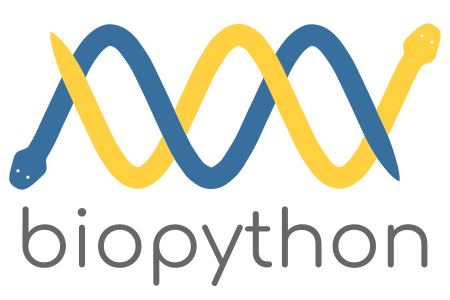
\includegraphics[width=0.3\textwidth]{biopython_logo_s.png} \\
\vspace{3mm}Biopython Project Update 2018}
\author{
	\underline{Ben Fulton}\thanks{Research Technologies, Indiana University, Bloomington, Indiana. Email: \href{mailto:befulton@iu.edu}{befulton@iu.edu}},
    Christian Brueffer\thanks{Department of Clinical Sciences, Lund University, Lund, SE},
    Peter Cock\thanks{Information and Computational Sciences, James Hutton Institute, Invergowrie, Dundee, UK},\\
    and the Biopython Contributors\thanks{See \href{https://github.com/biopython/biopython/blob/master/CONTRIB.rst}{contributor listing on GitHub}.}}
\date{19\textsuperscript{th} Bioinformatics Open Source Conference (BOSC) 2018, Portland, USA}

\begin{document}
\maketitle
\thispagestyle{empty}

\vspace{-0.2in}
\noindent
Website: \url{http://biopython.org} \\
Repository: \url{https://github.com/biopython/biopython} \\
License: Biopython License Agreement (BSD like, see \url{http://www.biopython.org/DIST/LICENSE}) \\

The Biopython Project is a long-running distributed collaborative effort,
supported by the Open Bioinformatics Foundation, which develops a freely
available Python library for biological computation \cite{AppNote}.
We present here details of the planned Biopython releases in 2018. 
Since the 1.70 release 
became available in July 2017, 55 unique users have contributed code 
fixes or enhancements, including 32 newcomers. This reflects our policy of
trying to encourage even small contributions.

2018 is expected to see the release of three new Biopython releases: 1.71, 1.72, and 1.73. The first is expected to be available in April 2018, and will include Python 3-compatible rich 
comparison for all Bio.PDB objects, helping to unify the API and easing sorting.
It also provides several new options and fixes for parsing and writing files, 
including PIR format for sequences, mmCIF files, and Gene files. In addition,
new codon tables 27-31 from NCBI (NCBI genetic code table version 4.2) were added.
This release will also include updated HTML
documentation based on the Sphinx documentation generator.

A further release, Biopython 1.72, is expected in the summer of 2018, and, if warranted, a final release for the year sometime in the fall.

In 2017 we started a re-licensing plan, to transition away
from our liberal but unique \emph{Biopython License Agreement} to the similar
but very widely used \emph{3-Clause BSD License}. We are in the process of 
reviewing the code base authorship file-by-file, in order to gradually dual 
license the entire project.

All releases fix miscellaneous bugs, enhanced the test suite,
and continued efforts to follow the PEP8 and PEP257 coding style guidelines
which is now checked automatically with GitHub-integrated continuous integration
testing using \href{https://travis-ci.org/biopython/biopython/builds}{TravisCI}.
We now also use \href{https://ci.appveyor.com/project/biopython/biopython/history}{AppVeyor}
for continuous integration testing under Windows.
Current efforts include improving the unit test coverage, which is easily viewed
online at \href{https://codecov.io/github/biopython/biopython/}{CodeCov.io}.

\begin{thebibliography}{}

\bibitem[Cock {\it et al}., 2009]{AppNote}Cock, P.J.A., Antao, T., Chang, J.T., Chapman, B.A., Cox, C.J., Dalke, A., Friedberg, I., Hamelryck, T., Kauff, F., Wilczynski, B., de Hoon, M.J. (2009) Biopython: freely available Python tools for computational molecular biology and bioinformatics. {\it Bioinformatics} {\bf 25}(11) 1422-3. \href{http://dx.doi.org/10.1093/bioinformatics/btp163}{doi:10.1093/bioinformatics/btp163}

\end{thebibliography}

\end{document}
